%! Author = Saeid Yazdani
%! Date = 11/26/2023


\section{The Trend in The Semiconductor Industry}
\label{sec:trend-semiconductor-industry}

For half a century, Moore’s Law was the promise
in the semiconductor industry stating that \enquote{the future of
the integrated circuits will be the future of electronics itself}
\autocite{moore} and by extrapolating available statistics concerning the number
of components per function per year, predicted doubling of the number of
integrated components per year (\autoref{fig:moore-trend}).

\begin{figure}[h]
    \centering
    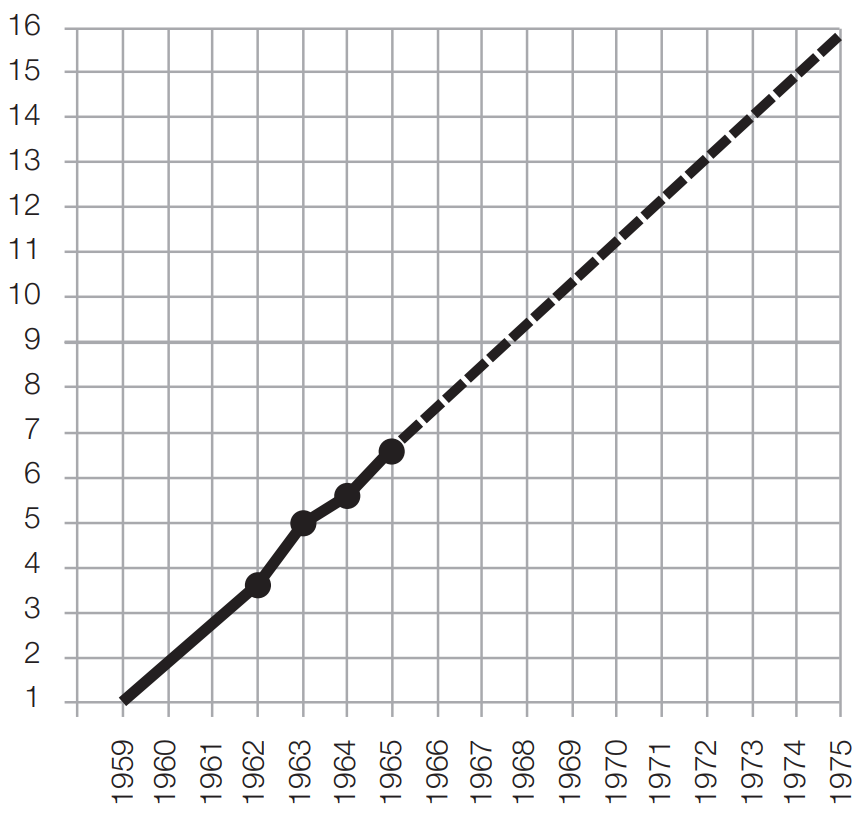
\includegraphics[width=0.62\linewidth,height=0.35\textheight,keepaspectratio]
    {figures/moore_extapolate}
    \caption[Moore's Law trend]{The Moore's Law trend. $ \log^{2} $ of the
    number of components per integrated functions \autocite{moore}}
    \label{fig:moore-trend}
\end{figure}

The data presented in \autoref{fig:moore-trend} was a generalized concept.
Between 1959 and 1965, there were no traces of microprocessors.
What is now referred to as Moore's Law is likely the interpretation of
Dennard's scaling rule \autocite{bohr} and the name itself did not appear
in the general public until 1979 \autocite{mollic}.
Regardless, this assumption remained true for most computing integrated circuits
based on \ac{CMOS} technology \autocite{benedictis}.

Today, we are facing the energy conservation challenge, and highly
efficient power converters are a prerequisite in many application areas such as
\ac{IoT} devices, online sensors, and monitoring systems where energy
efficiency and long battery life is mandatory \autocite{bahai}.

\ac{CMOS}-based integrated circuits have reached high
speed and lower power within decades.
Smart Power cannot be made from \SI{5}{\nano\meter} technology; therefore,
\SI{35}{\nano\meter} to \SI{70}{\nano\meter} technologies are on the rise again
as shown in \autoref{fig:wafer-size-evolution}.

While modern \acs{CPU}s, \acs{GPU}s and \acs{ASIC}s are heading to
the sub \SI{10}{\nano\meter} processes, other categories of
integrated circuits, such as power converters, are not following the same trend
\autocite{masuda}.

Production cost is a critical factor in integrated
circuits.
For this reason, the industry increased wafer
area, resulting in reduced costs per function or silicon area.
While $3\,''$ wafers (\SI{76}{\milli\meter}) were prominent in the 1970s,
currently $12\,''$ wafers (\SI{300}{\milli\meter}) are state of
the art as depicted in \autoref{fig:wafer-size-evolution}.

A transition to larger wafer sizes that should have increased the yield and
throughput had to be stopped, as it required a tremendous amount of
investment and cost, which may take a long time for the initial investment to
pay off.

So far, there have been unsuccessful attempts to develop
$18\,''$ (\SI{450}{\milli\meter}) wafers.
An $18\,''$ wafer would have more than two times the area of a $12\,''$ wafer,
but the associated costs for producing machinery at this diameter have not yet
made it economical to become a new standard for wafer size.

\begin{figure}[htbp]
    \centering
    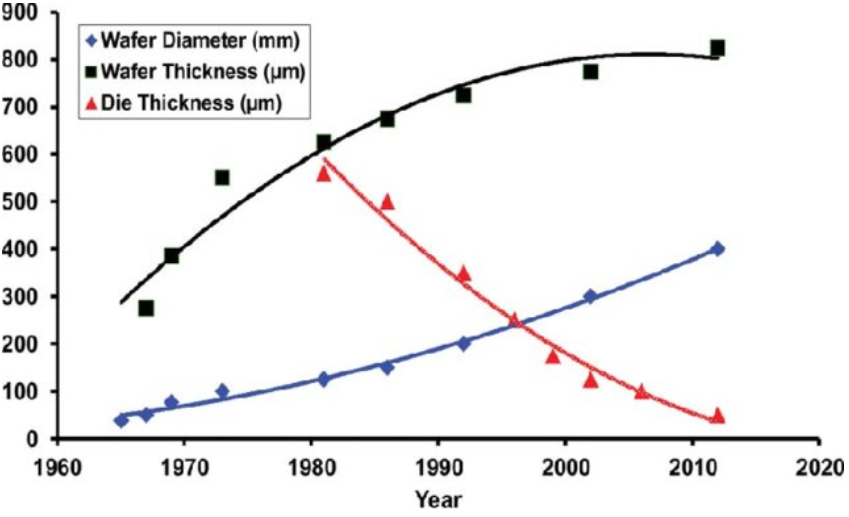
\includegraphics[width=0.84\linewidth,height=0.50\textheight,keepaspectratio]
    {figures/wafer-trend}
    \caption[Waver technology evolution over time]{Evolution of wafer diameter
    over time in comparison with wafer thickness and die thickness
    \autocite{RajMarks}.}
    \label{fig:wafer-size-evolution}
\end{figure}
